
\section{Methodology}

\subsection{Strip and Bind} \label{methodo:est}

\begin{figure}[t!]
 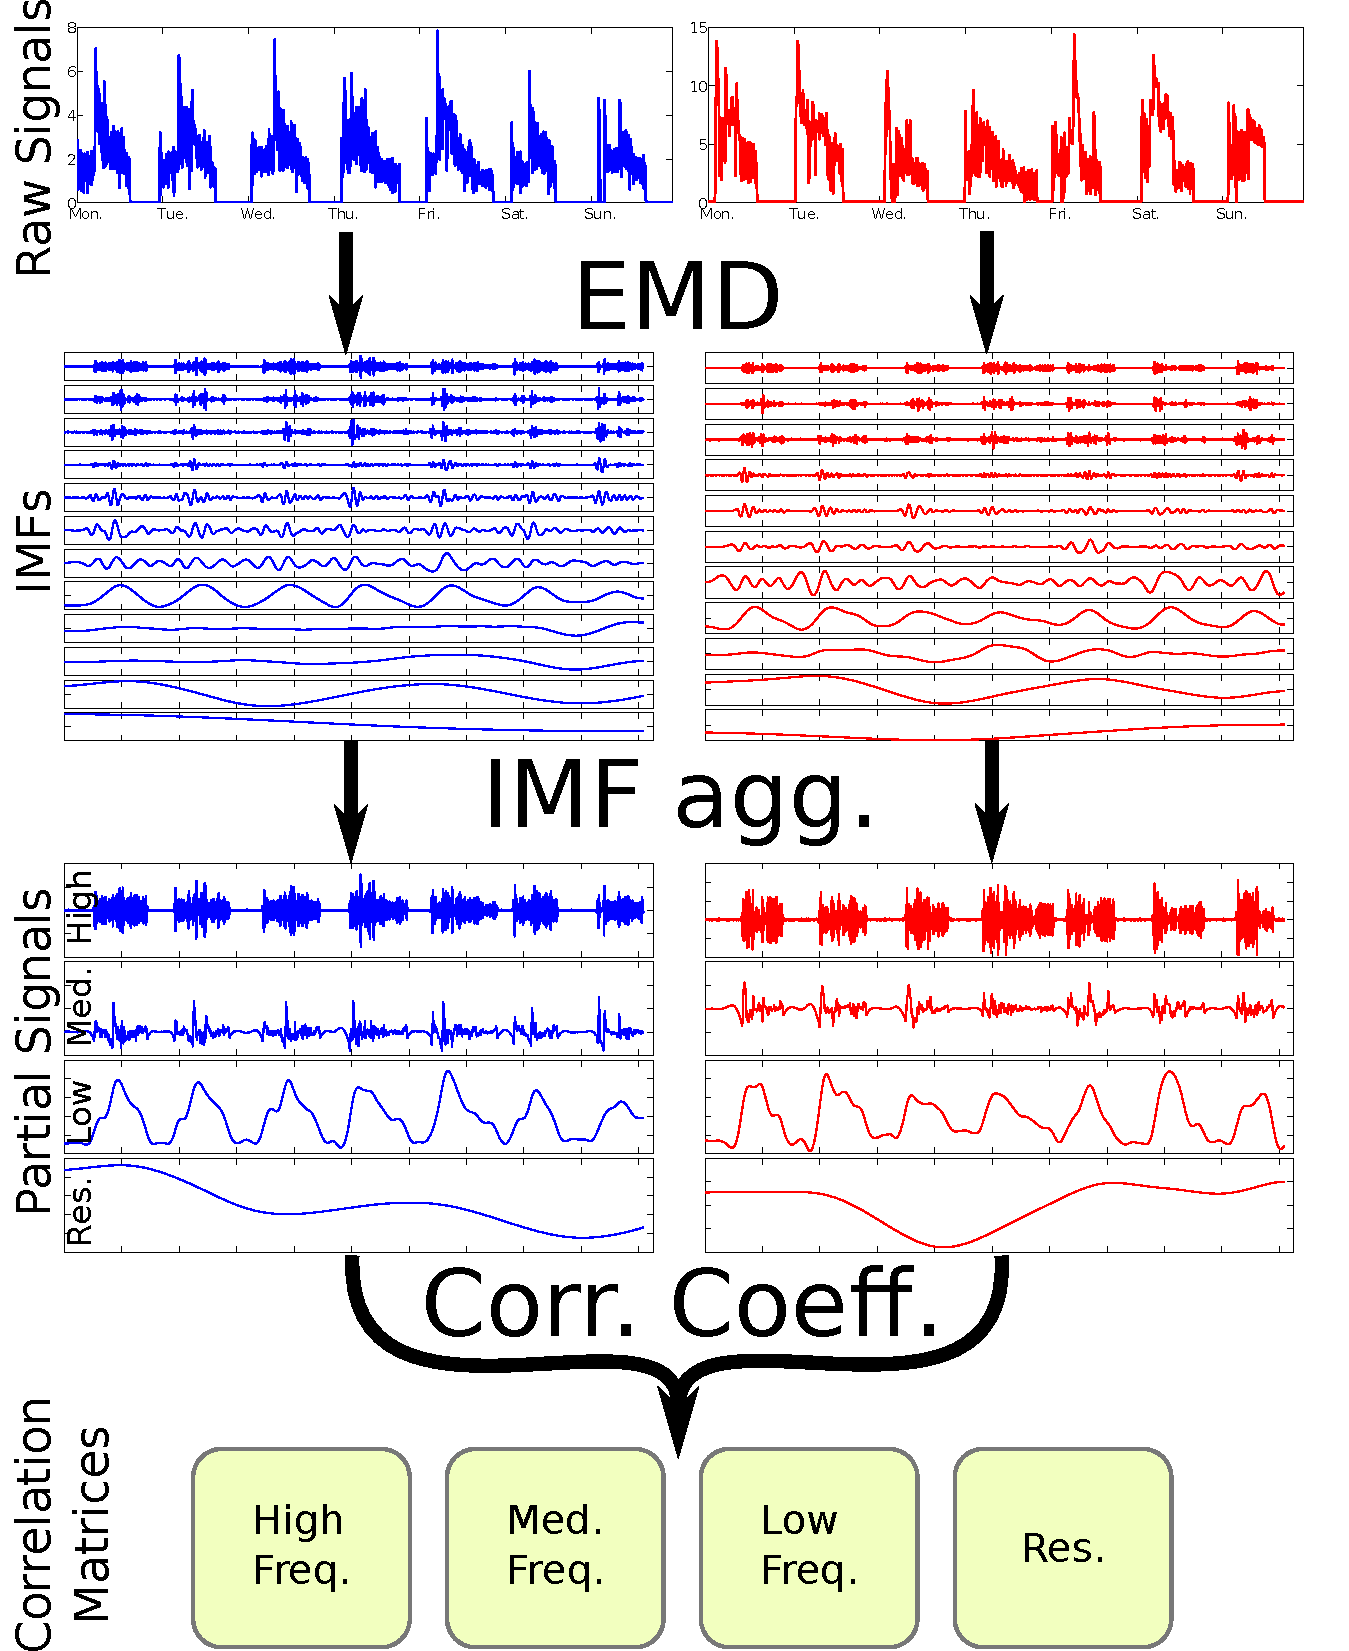
\includegraphics[width=.5\textwidth]{img/estimator.pdf}
 \caption{\emph{Strip and Bind} using two raw signals standing for one week of data from two different HVACs. (1)~Decomposition of the signals in IMFs using EMD (top to bottom: $c_1$ to $c_n$); (2)~aggregation of the IMFs based on their time scale; (3)~comparison of the partial signals (aggregated IMFs) using correlation coefficient.}
 \label{fig:diagram1}
\end{figure}

%As shown in the previous section, discovering the devices that are used in concert is particularly difficult.
Discovering devices that are used in concert is non-trivial.  
SBS decomposes each signal into an additive set of components, called Intrinsic mode functions (IMF), 
that decomposes the signal into sub-signals at different time scales.  IMFs are obtained using 
%that reveal the signal structures at different time scales.
Empirical Mode Decomposition (see Fig.~\ref{fig:diagram1} and Section~\ref{emd}).
%Then, we filter out the IMFs that interfere with our goal and keep only those standing for time scales shorter than the unwanted daily pattern.
%We then remov out IMFs with time scales 
We only consider IMFs with a daily time scale or smaller, since we are interested in capturing short-scale dependencies
for services being delivered.
Consequently, SBS aggregates the IMFs that falls into the same relative time scales ranges (see \emph{IMF agg.} in Fig.\ref{fig:diagram1}).
%The resulting partial signals of different devices are compared pairwise to identify the devices intrinsic relationships (see \emph{Corr. Coeff.} in Fig.\ref{fig:diagram1}). 
The resulting partial signals of different device power traces are compared, pairwise, to identify the devices that show un/correlated patterns at different time scales (see \emph{Corr. Coeff.} in Fig.\ref{fig:diagram1}).


% These intrinsic relations are uncovered by comparing the sensors data at certain meaningful frequency bands.
% Namely, looking at high frequency allows to compare short-term variations representing the instantaneous devices change of state, however, the low frequency highlights long-term fluctuations revealing long devices usage pattern.
% 
% ..... the similarity estimators analyzes the readings from several sensors and reports scores standing for the similarity of the sensors at different frequency bands.
% First, the similarity estimator takes advantage of EMD to decompose the sensors signals into a set of components called intrinsic mode functions (IMFs).
% Second, it constructs band-limited signals by aggregating the IMFs whose mean frequencies fall in a certain frequency band.
% Thereby the pairwise comparison of band-limited signals provides the sensors correlations at different frequency bands. 
% 
% The advantages of the proposed intrinsic-correlation estimator are adaptive approach, ... 

% These two steps are described by the two following sections.

\subsubsection{Empirical Mode Decomposition} \label{emd}
Empirical Mode Decomposition (EMD) \cite{huang:emd1998} is a technique that decomposes a signal and reveals its intrinsic patterns, 
trend and noise.
This technique has been widely applied to a variety of datasets, including climate variables~\cite{lee:climateEMD2011}, medical data~\cite{blanco:bioMed2008}, speech signals~\cite{huang:signalProc2006,hasan:ieeeletter2009}, and image processing~\cite{nunes:vision2005}.
% for example, it helped to uncover the global surface temperature trends\cite{}, solar activity patterns and predicts climate variables .
EMD's effectiveness relies on its empirical, adaptive and intuitive approach.
In fact, this technique is designed to efficiently decompose both non-stationary and non-linear signals without requiring any 
a priori basis functions or tuning.  

EMD decomposes a signal into a set of oscillatory components called intrinsic mode functions (IMFs). 
An IMF satisfies two conditions: (1) it contains the same number of extrema and zero crossings (or differ at most by one); (2) the two 
IMF envelopes defined by its local maxima and local minima are symmetric with respect to zero.  Consequently, 
 IMFs are functions that directly convey the amplitude and frequency modulations.

% EMD is an iterative sifting process that extracts IMFs step by step; each step seeks for the IMF with the highest frequency, then the computed IMF is removed from the data and the residual data are used as input for the next step.
EMD is an iterative algorithm that extracts IMFs step by step by using the so-called sifting process \cite{huang:emd1998}; each step seeks for the IMF with the highest frequency by sifting, then the computed IMF is removed from the data and the residual data are used as input for the 
next step.
The process stops when the residual data becomes a monotonic function from which no more IMF can be extracted.

We formally describe the EMD algorithm as follows: 
\begin{enumerate}
\item For a signal \emph{X(t)}, let $m_0$ be the mean of its upper and lower envelopes as determined from a cubic-spline interpolation of local maxima and minima.
\item The first component $h_0$ is computed: $h_0=X(t)-m_0$
\item  The Sifting process is iterated, $h_1$ taking the place of $h_0$. Using its upper and lower envelopes, a new local mean $m_1$ is computed and $h_2 = h_1-m_1$.
\item The procedure is repeated $k$ time until $h_k=h_{k-1}-m_{k-1}$ is an IMF according to the two conditions above.
\item Then it is designated as $c_1=h_{k}$, the first IMF from the data, which contains the shortest period component of the signal. We separate it from the rest of the data: $X(t)-c_1 = r_1$, and the procedure is
repeated on $r_j: r_1-c_2 = r_2,\dots,r_{n-1} - c_n = r_n$
\item The process stops when residual $r_n$ contains no more than 3 extrema.
\end{enumerate}

The result of EMD is a set of IMFs $c_i$ and the final residue $r_n$, such as: \[X(t)=\sum^{n}_{i=1}c_i+r_n\]
where the size of the resulting set of IMFs $n$ depends on the original signal $X(t)$ and $r_n$ represents the trend of 
the data (see \emph{IMFs} in Fig.\ref{fig:diagram1}).

For this work we implemented a variant of EMD called Complete Ensemble EMD~\cite{torres:icassp2012}.
This algorithm computes EMD several times with additional noise, it allows us to efficiently analyze signals that have 
flat sections (i.e. consuming no electricity in our case). % and permits us to solve the \emph{EMD mode mixing problem}.

\subsubsection{IMF aggregation} \label{methodo:corr}
By applying EMD to energy consumption signals we obtain a set of IMFs that precisely describe the devices consumption 
patterns at different time scales.  Therefore, we can focus our analysis on the smaller time scales, ignoring the dominant 
patterns that prevent us from effectively analyzing raw signals.

However, comparing the IMFs obtained from different signals is also not trivial,
 because EMD is empirically uncovering IMFs from the data there is no guarantee that the two IMFs $c_i^1$ and $c_i^2$ obtained from two distinct signals $S^1$ and $S^2$ represent data at the same frequency domain.
Directly comparing $c_i^1$ and $c_i^2$ is meaningless unless we confirm that they belongs to the same frequency domain.

There are numerous techniques to retrieve IMF frequencies~\cite{huang:aada2009}.  
In this work we take advantage of the Generalized Zero Crossing (GZC)~\cite{huang:patent2006} because it is a simple and robust 
estimator of the IMF instantaneous frequency \cite{huang:aada2009}.
GZC is a direct estimation of IMF instantaneous frequency using critical points defined as the zero crossings and local extrema 
(round dots in Figure \ref{fig:gzc}).
Formally, given a data point $p$ GZC measures the quarter ($T_4$), the two halves ($T_2^x$) and the four full periods ($T_1^y$) $p$  belongs to (see Figure \ref{fig:gzc}) and the instantaneous period is computed as:
\[T=\frac{1}{7}\{4T_4+(2T_2^1+2T_2^2)+(T_1^1+T_1^2+T_1^3+T_1^4)\}\]

\begin{figure}
\begin{center}
 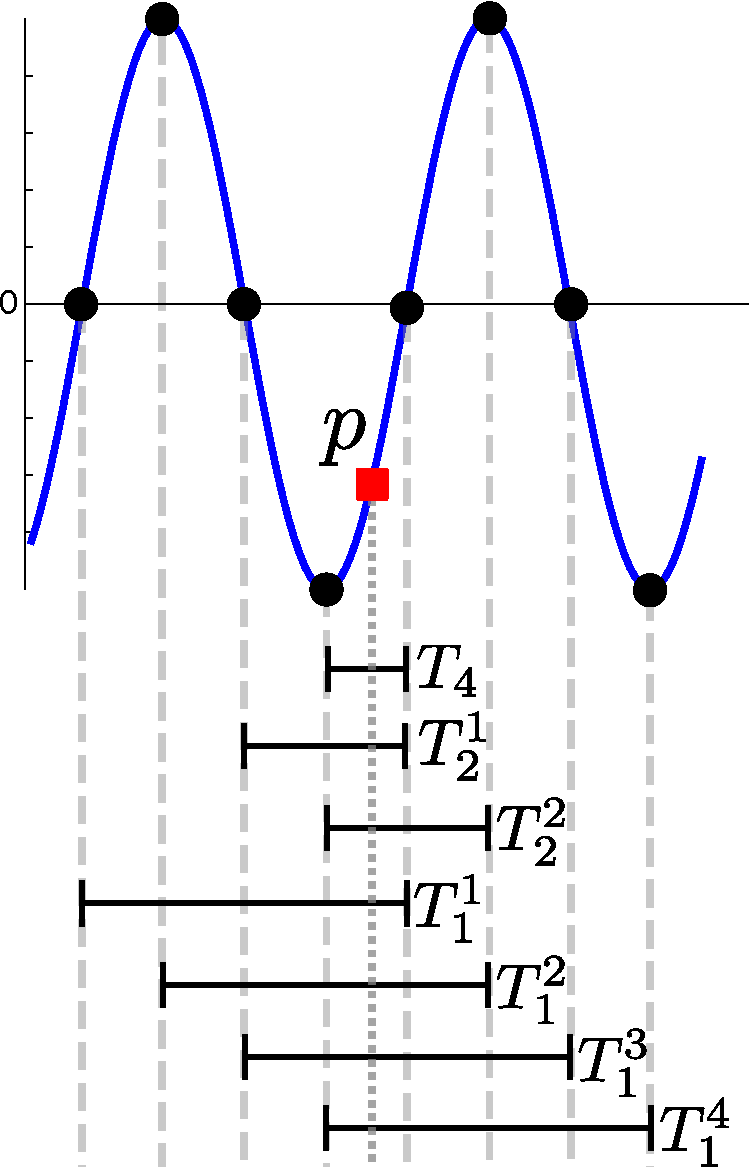
\includegraphics[width=.25\textwidth]{img/gzc.pdf}
 \end{center}
 \caption{Generalized Zero Crossing: the local mean period at the point $p$ is computed from one quarter period $T_4$, two half periods $T_2^x$ and four full periods $T_1^y$ (where $x=1, 2$, and, $y=1,2,3,4$).}
 \label{fig:gzc}
\end{figure}

Since all points $p$ between two critical points have the same instantaneous period GZC is local down to a quarter period.
Hereafter, we refer to the time scale of an IMF as the average of the instantaneous periods along the whole IMF.
Because the time scale of each IMF depends on the original signal, we propose the following, to efficiently compare IMFs from different signals.
We cluster IMFs with respect to their time scales and partially reconstruct each signal by aggregating its IMFs from the 
same cluster.  Then, we directly compare the partial signals of different devices.

The IMFs are clustered using four time scale ranges: 
\begin{itemize}
 \item The \emph{high frequencies} stand for all the IMFs with a time scale lower than 20 minutes. These IMFs capture the noise.
 \item The \emph{medium frequencies} stand for all the IMFs with a time scale between 20 minutes and 6 hours. These IMFs convey the detailed devices usage.
 \item The \emph{low frequencies} stand for all the IMFs with a time scale between 6 hours and 6 days. These IMFs represent the daily pattern of the devices.
 \item The \emph{residual data} is all data with a time scale higher than 6 days. This is mainly the residual data obtained after applying EMD and it highlights the trend of the devices.
\end{itemize}

These time scale ranges are chosen based on our experiments and goal.
The 20-minute boundary relies on the sampling period of our dataset (5 minutes) and permits us to capture IMFs with really short periods.
The 6-hour boundary allows us to analyze all patterns that have a period shorter than the usual office hours.
The 6-day boundary allows us to capture daily patterns and weekday pattern.

Aggregating signal IMFs, within each time scale range, results in 4 partial signals representing different characteristics of the device's
 energy consumption (see \emph{Partial Signals} in Fig.\ref{fig:diagram1}).
We do a pairwise device trace comparison, calculating the correlation coefficient of their partial signals.
In the example shown in Figure~\ref{fig:diagram1}, the correlation coefficient of the raw signals suggests that they are highly correlated ($0.57$). 
However, the comparison of the corresponding \emph{partial signals} provides new insights;
the two devices are poorly correlated at high and medium frequencies (respectively $-0.01$ and $-0.04$) but highly correlated at low frequencies ($0.79$) meaning that these devices are not ``intrinsically'' correlated.  They only share a similar daily pattern.

All the devices are compared pairwise at the four different time scale ranges.
Consequently, we obtain four correlation matrices that convey the device similarities at different time scales.
Each line of these matrices (or column, since the matrices are symmetric) reveals the behavior of a device -- its relationships with the 
other devices at a particular time scale.
The matrices form the basis for tracking the behavior of devices and to search for misbehavior.


\subsection{Search}\label{methodo:ano}
\emph{Search} aims at identifying misbehaving devices in an unsupervised manner.
Device behavior is monitored via the correlation matrices presented in the previous section.
Using numerous observations SBS computes a specific reference that exhibits the normal inter-device usage pattern.
Then, SBS compares the computed reference with the current data and reports devices that deviate from their usual 
behavior.

\subsubsection{Reference}
We define four reference matrices, which capture normal device behavior at the four time scale ranges defined in 
Section~\ref{methodo:corr}.
The references are computed as follows: (1) we retrieve the correlation matrices for $n$ consecutive time bins (as described in Section~\ref{methodo:est}). (2) For each pair of devices we compute the median correlation 
over the $n$ time bins and obtain a matrix of the median device correlations.

Formally, for each time scale range the computed reference matrix for $d$ devices and $n$ time bins is:
\[R_{i,j} =  \median(C^1_{i,j},...,C^n_{i,j})\]
where $i$ and $j$ ranges in $[1,d]$.

% Assuming that device-usage predominantly behaves normally and the anomalies are exceptional 
% events, the reference matrices exhibit the normal device behaviors.
Our model assumes anomalies are rare and the majority of the data is normal.
This is a common assumption in unsupervised anomaly detection.
% We assume that normal behavior is not truly anomalous.
Abnormal correlation values, that could appear during model construction, %in the analyzed time bins 
are ignored by the median operator thanks to its robustness to outliers (50\% breakdown point).  
However, if that assumption does not hold (more than 50\% of the data is anomalous), our model will flag the opposite -- labeling abnormal as normal and vice-versa.
From close inspection of our data, we believe our primary assumption is sound.
% Normal behavior occurs most frequently, therefore detected anomalies should be meaningful.



\subsubsection{Behavior change}
% SBS consists in identifying the devices that significantly deviate from their normal behaviors as defined in the reference matrices.
% Consequently, 
We compare each inter-device usage matrix, for all time bins, to the one provided by the reference matrix.  
Consider the correlation matrix $C^t$ obtained from the data for time bin $t$ ($1 \leq t \leq n$).  
Vector $C^t_{i,*}$ is the behavior of the $i^{th}$ device for this time bin.
Its normal behavior is given by the corresponding vector in the reference matrix $R_{i,*}$.
We measure the device behavior change at the time bin $t$ with the following Minkowski weighted distance:
\[ l^t_{i} = \left(\sum_{j=1}^d  w_{ij}\left(C^t_{i,j} - R_{i,j}\right)^p\right)^{1/p} \]
where $d$ is the number of devices and $w_{ij}$ is:
\[ w_{ij} = \frac{R_{i,j}}{\sum_{k=1}^d R_{i,k}}. \]
The weight $w$ enables us to highlight the relationship changes between the device $i$ and those related to it in the reference matrix.
In other words, our definition of behavior change is mainly driven by the relationship among devices that are usually highly correlated.
We also set $p=4$ in order to inhibit small differences between $C^t_{i,j}$ and $R_{i,j}$ but emphasize the important ones.

By monitoring this quantity over several time bins the abnormal device behaviors are easily identified as the outlier values.
In order to identify these outlier values we implement a robust detector based on median absolute deviation (MAD), a dispersion measure commonly used in anomaly detection \cite{huber:wiley2009,chan:springer2005}.
It is a measure that robustly estimates the variability of the data by computing the median of the absolute deviations from the median of the data.
 Let $l_{i} = [l_i^1,...,l_i^n]$ be a vector representing the behavior changes of device $i$ over $n$ time bins, then its MAD value is defined as:
\[ \mad_i = b \median(\lvert l_{i} - \median(l_{i})\rvert)\]
where the constant $b$ is usually set to $1.4826$ for consistency with the usual parameter $\sigma$ for Gaussian distributions.
Consequently, we define anomalous behavior, for device $i$ at time $t$, such that the following equation is satisfied:%of the device $i$ at the time bin $t$ that satisfies the following equation:
\[l^t_{i} > \median(l_{i}) + \tau  \mad_i\]
Note, $\tau$ is a parameter that permits to make SBS more or less sensitive.

The final output of SBS is a list of alarms in the form $(t,i)$ meaning that the device $i$ has abnormal behavior at the time bin $t$.
The priority of the alarms in this list is selected by the building administrator by tuning the parameter $\tau$.
